%\addcontentsline{toc}{chapter}{Development Process}
\chapter{Design}
The design for the system was completed in two major steps. First, the initial design was created before any development and secondly, incremental changes were made to add more detail to the design with every relevant feature. The initial design formed the overall model for the system, and was only added to over the duration of the project. The UML class diagrams were designed to be basic initially, and only contained major functions and classes. These then evolved as the features were developed. The diagrams displayed in this section will be the final full diagrams.

At the \textbf{Plan by Feature} level, design was performed at the start of each feature. A feature would be analysed, and the relevant functions and variables that were required, would be added to the design first. Following this, unit (or system) tests would be designed to exercise the functions, as well as the full requirements of the feature.

\newpage

\section{Informing the Overall model}
\subsection{Use case}

\begin{figure}[h!]
	\centering{
		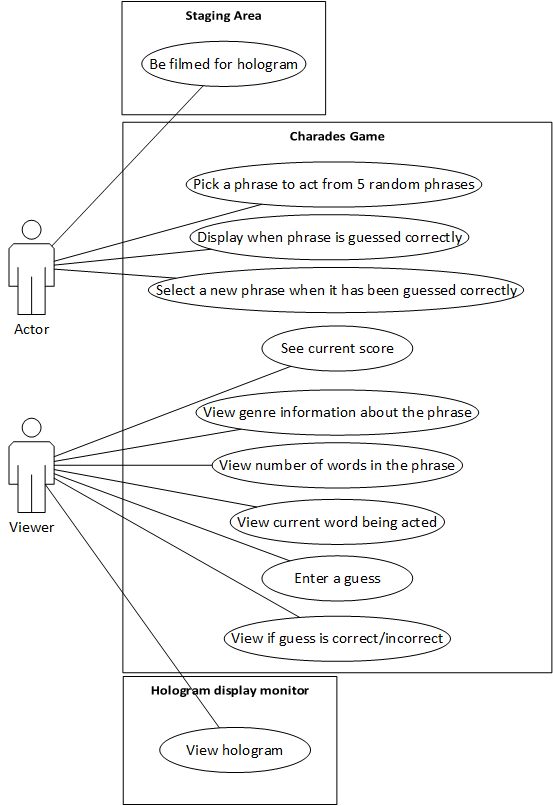
\includegraphics[scale=0.75]{Chapter2/use_case.png}
		\caption{A use case diagram to show how the users will interact with the system and the functionality they require.}
		\label{fig:use_case}
	}
\end{figure}

To best identify the requirements of the users, the use case diagram (Figure \ref{fig:use_case}) was produced. In addition to the functionality required by each type of user (Actors and Viewers), the diagram also divides the system into basic sub systems. This diagram was an insightful first step in the early development of the system as it gave an overview of the system as a whole, prior to any major implementation choices being required. Whilst the diagram was basic, it showed the interactions that users would have with the system. These interactions formed the input and output requirements that needed to be addressed in the user interface design. In addition, the use case diagram showed that the Charades game functionality is dependant on the whether the user is an actor or a viewer. This in turn promoted a model-view-controller design pattern to be used for the system.

\newpage

\subsection{Activity diagram}

\begin{figure}[h!]
	\centering{
		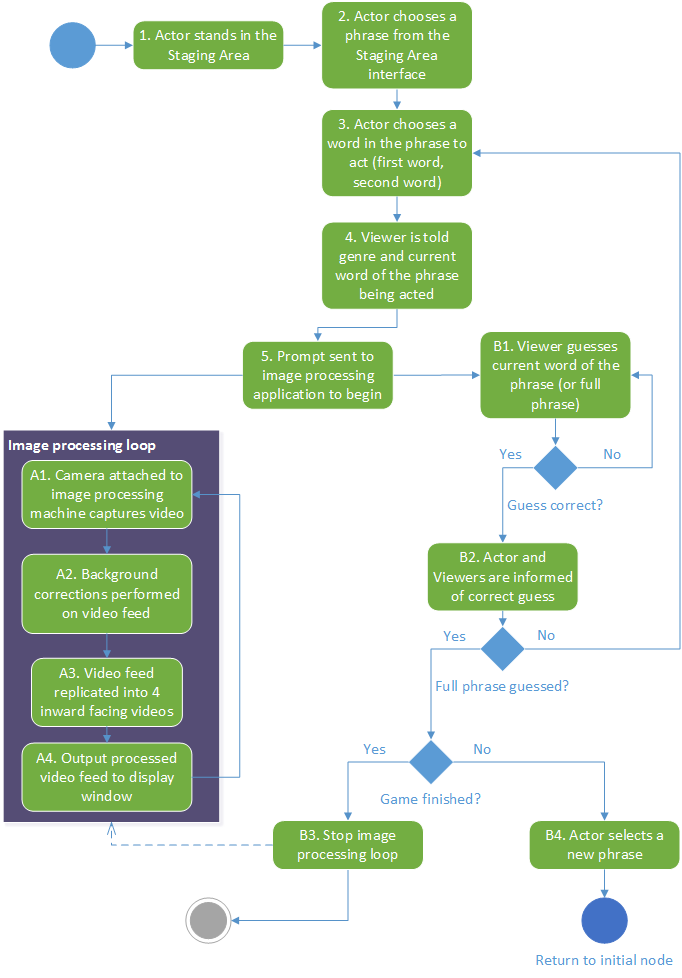
\includegraphics[scale=0.70]{Chapter2/activity_diagram.png}
		\caption{An activity diagram that describes the flow of information in the system. It includes the data flow for both the Hologram and Charades systems.}
		\label{fig:activity_diagram}
	}
\end{figure}

Given the system was designed to be a game of charades, it follows a linear set of instructions that mirror the original rules of the charades game. An activity diagram was chosen to model the flow of activities in the system, due to the well defined path of game play. Figure \ref{fig:activity_diagram} shows an activity diagram that maps the basic flow of a single round of the game. The \textit{Image processing loop}, shown in purple, describes the flow  of the hologram creation. This process (prefixed with the letter A) runs continuously in parallel with the game loop (prefixed with the letter B).

\subsection{Component diagram}

\begin{figure}[h!]
	\centering{
		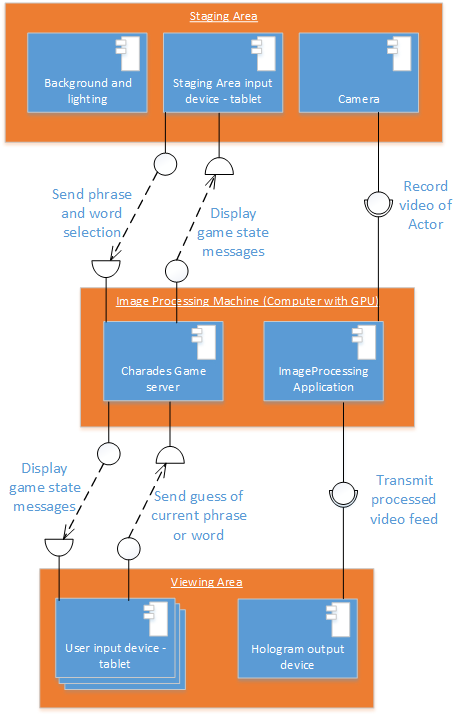
\includegraphics[scale=0.80]{Chapter2/component_diagram.png}
		\caption{A component diagram that describes both the software and hardware components of the system, and how they interact with each other.}
		\label{fig:component_diagram}
	}
\end{figure}

The system, in its totality, had to include multiple pieces of hardware in order to operate. The component diagram, shown in Figure \ref{fig:component_diagram}, helped to combine the different hardware considerations in tandem with the software. Furthermore, the diagram confirmed the presence of three separate major entities in the project.

The \textbf{Staging Area} would be where the actor would be filmed. The camera directly connects to the Image Processing machine via a USB cable for data transfer. The Staging Area input device will use a wireless connection to send and receive messages from the Charades Game server that is hosted on the Image Processing machine.

The \textbf{Image Processing machine} is a computer that acts as the server for the website, as well as running the image processing application for the holograms. Due to the nature of the video feed processing in real-time, the computer will require a Graphical Processing Unit (GPU). The Image Processing application receives input of the raw video feed from the camera in the Staging Area and will process the video, and output the result. The Charades Game server is hosted on the Image Processing machine. This component will handle the flow between the users in the Viewing Area and the Actor in the Staging Area.

The \textbf{Viewing Area} is the area where the Pepper's Ghost Pyramid and the monitor displaying the output of the hologram system are housed. The area will be a dark tent in order to produce the best quality (most visible) hologram.

\newpage


\section{Overall Architecture}
\subsection{Hologram creation system}

\begin{figure}[h!]
	\centering{
		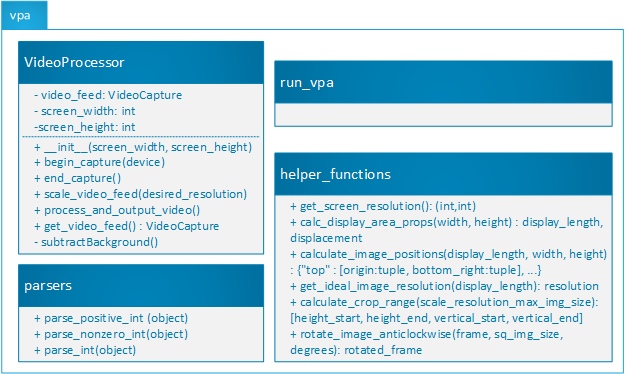
\includegraphics[scale=0.9]{Chapter2/vpa_class_diagram.png}
		\caption{The UML class diagram for the hologram creation system. The diagram shows the vpa module and the enclosed subclasses and submodules.}
		\label{fig:vpa_class_diagram}
	}
\end{figure}

\begin{itemize}
	\item \textbf{vpa}: This module holds all the code for hologram creation system. vpa stands for \textit{Video Processing Application} as the code in this module handles the processing of the video feed.

	\item \textbf{run\_vpa}: This is a script and is the most simplistic in the module. It is the driver script for the VideoProcessor class and runs the required functions to begin the video feed capture and display the manipulated video feed in the output window.

	\item \textbf{parsers}: This module holds several functions that are used to ensure that values provided in the system are expected and correct. As Python is not a strongly typed language, the parsers are required to ensure that no type errors occur during execution of the application. The parser functions have been separated into their own module to group them together. All functions in the parser module receive input of a single Object (where Object is the super class of all Python variables) and will raise a Python ValueError if they do not meet the criteria of the function.

	\item \textbf{VideoProcessor}: This class handles the main functionality and logic of the application. The most important function in the VideoProcessor is the process\_and\_output\_video function. This function contains the main processing loop of the application. This loop will call the functions that handle the scaling, rotation and positioning of the video feed. These functions are located in the helper\_functions module.  

	\item \textbf{helper\_functions}: This module was not present in the original design, but in order to improve the quality, readability and test coverage of the code, it was added to hold refactored code from the \textbf{VideoProcessor} class. In addition to providing simple helper functions, such as obtaining the screen resolution and calculating the size of the display window relative to the centre of the screen, the helper\_functions module also aids with manipulation of the video feed. Functions used for calculating the location, cropping and rotation of the image are also in the helper\_functions module.

\end{itemize}

The VideoProcessor has been designed as a class rather than a collection of functions so that the video\_feed variable (which contains the video feed from the web cam) can be stored.

\newpage

\subsection{Charades Game}
\subsubsection{Model Design}
\begin{figure}[h!]
	\centering{
		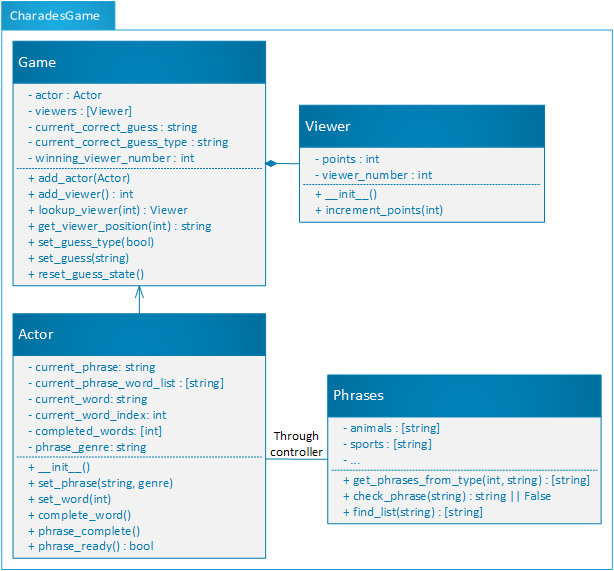
\includegraphics[scale=0.9]{Chapter2/charades_class_diagram.png}
		\caption{The UML class diagram for the model of the Charades Game.}
		\label{fig:charades_class_diagram}
	}
\end{figure}

Figure \ref{fig:charades_class_diagram} shows the design for the Model used to represent data in the Charades game. For the Model, it was decided not to use a database and instead use a class representation for data storage. The reasoning behind this is that the flow of the charades game is dependant on the state of the system, and a class based model provides a better way to model state versus a database alternative.\\
The Model has been separated into four files:

\begin{itemize}
	\item \textbf{Game}: The Game class holds the state of the game at its highest level of abstraction. As well as holding a list of the Viewers and Actors, the Game also holds information regarding the whether or not a correct guess has been made, the type of the guess and the viewer\_number of the winner for the round. All of these values are used to update the game state and inform the users of the current state of the game via the APIs.
	
	\item \textbf{Viewer}: The Viewer is a simple class that holds the number of points accumulated by a viewer, and the unique viewer\_number of that viewer. When a viewer logs in, the viewer\_number is automatically generated and assigned to a Viewer object which is added to the Game object. In addition to the Viewer being created in the model, the viewer\_number is also stored client side in a session cookie. This viewer\_number is then queried when the client needs to display a viewers score. 
	
	\item \textbf{Actor}: The Actor class holds the current phrase and word variables for the phrase that is being acted. The model uses the concept of phrases and words for topics that an Actor will select to act out. In this scenario, a phrase is the whole topic that is being acted, for example "Shot put". However, a word is part of a phrase, for example "Shot" is a word in the phrase "Shot put". In addition it has functions to set new words and phrases and complete words when they are guessed correctly.
	
	\item \textbf{Phrases}: The Phrases module holds all the phrases that can be acted by the Actor in Python lists. In addition, the module contains several helper functions designed to check phrases exist in the list of known phrases and to acquire a phrase, at random, from the list.
	
\end{itemize}

The phrase section of the model could have been improved by using a database representation. This data, unlike that of the other classes in the model, remains static and could therefore be more suited to using a simple database to hold the information. However, a possible caveat for this is the addition of another technology to the model. Whilst this technology would be simple and is well supported, it would add some additional complexity compared to using the same method as the class representation.

\newpage

\subsubsection{Routing and Website Design}
\begin{figure}[h!]
	\centering{
		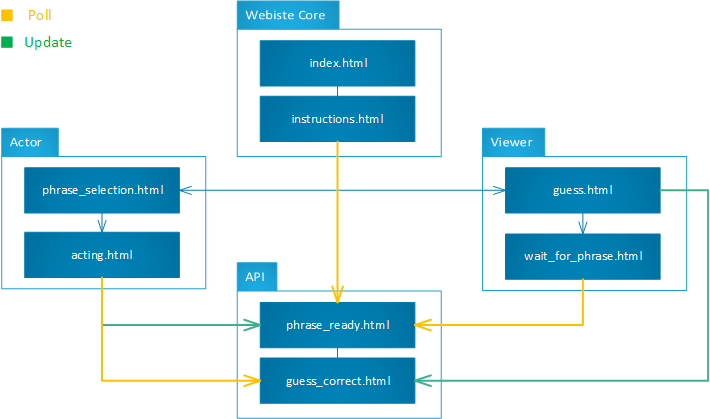
\includegraphics[scale=0.75]{Chapter2/website_design.png}
		\caption{The website design for the Charades Game. The diagram shows the Template structure of the website, as well as when pages are updated from the API and when polling of the API takes place.}
		\label{fig:website_design}
	}
\end{figure}

Figure \ref{fig:website_design} shows the design for the templates (html pages) of the website. The web pages are grouped into relevant sections that relate to their functionality:

\begin{itemize}

	\item \textbf{Website Core}: The Website core includes the login (index) and instructions page. The index.html page is where the user will provide the session password (This would be provided on the day that the system is being used, or set up in advance for an event), and the option to login in as a Viewer or Actor. The instructions.html provides a dynamic set of instructions depending on the type of user (Actor or Viewer), and a 'continue' button for the Actor to continue to the phrase\_selection page. In addition, for a viewer, the page will poll the phrase\_ready API and, when true, display a button for viewers to click to advance to the next section of the website.
	
	\item \textbf{Actor}: The Actor section of the website handles phrase and word selection, as well as a default page for the actor to view while the current phrase is being acted. The phrase\_selection.html page provides the actor with a selection of five phrases and instructs them to select one. Once chosen, the actor advances to the acting.html page where the phrase is displayed, and, if the phrase contains multiple words, the actor is asked to choose a word from the phrase. Once the phrase and word have been selected, the phrase\_ready API will be updated to display True.
	
	\item \textbf{Viewer}: The Viewer section of the website handles correct or incorrect guesses of the words or phrases. The  guess.html page is where the viewers attempt to guess the current word or phrase being acted. Information about the genre, number of words and current word is also displayed to the viewer on this page, as well as a text field for viewers to submit their guesses (see Figure \ref{fig:guess_ui}). This page both polls and updates the guess\_correct API. When a correct guess has been made, the API is updated with either "Word" or "Phrase" depending on the guess type. As multiple users will be on this page, the page also polls the guess\_correct API to see if a correct guess has been made. When a correct guess has been made, both the viewer who guessed correctly and all other viewers are taken to the wait\_for\_phrase page. This page polls the phrase\_ready API and when a new phrase has been selected (the API returns 'True') viewers are redirected back to the guess.html page to guess the next word or phrase.
	
	\item \textbf{API}: The API consists of simple pages that are used when polling the game state for information. The phrase\_ready.html API displays 'True' when the phrase is in a guessable state (i.e. the phrase and word have been selected and the phrase or word have not been correctly guessed) and 'False' when not guessable. The guess\_correct.html API displays 'None' when no correct guesses have been made by the viewers, 'Word' when the word has been guessed correctly and 'Phrase' when the phrase has been correctly guessed.
	
\end{itemize}

\newpage

\subsection{UI Design}
\begin{figure}[h!]
	\centering{
		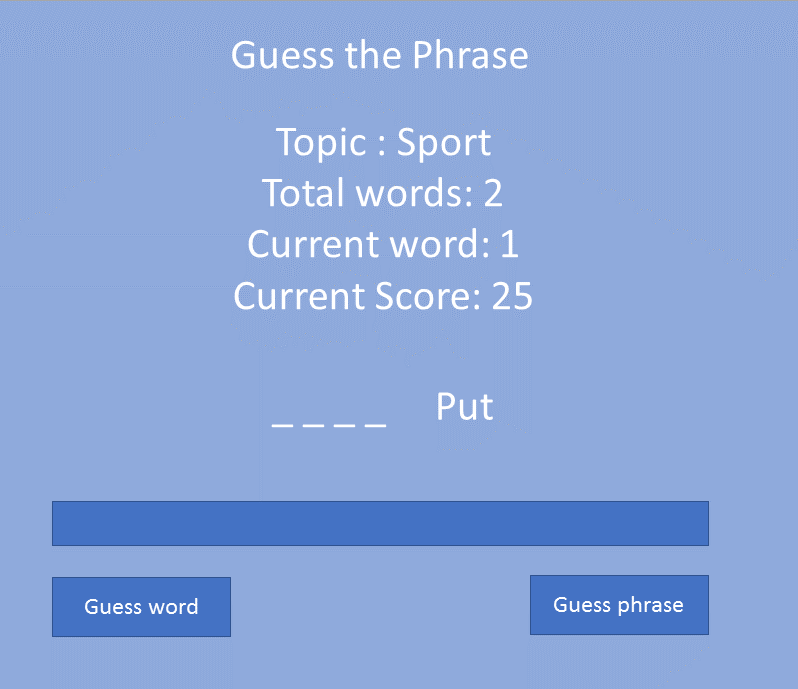
\includegraphics[scale=0.7]{Chapter2/guess_ui.png}
		\caption{The UI design for the guess.html page. This page shows a user with 25 points and the phrase "Shot put" is being acted. The word "Put" has already been guessed, meaning the word "Shot" is represented by '\_ \_ \_ \_' as it has yet to be guessed.}
		\label{fig:guess_ui}
	}
\end{figure}

Figure \ref{fig:guess_ui} shows the UI design for the viewers guess.html page (All other UI diagrams are available in Appendix D). The purpose of the UI diagrams was to ensure that all the functionality required for user interaction on a given page was met. In the case of Figure \ref{fig:guess_ui}, the page had to do the following:
\begin{itemize}
	\item Display the Genre information
	
	\item Display the total number of words in the phrase
	
	\item Display the current word being acted (when phrases contain multiple words)
	
	\item Display the viewers current score
	
	\item Provide a way for the viewers to submit a guess for the current word or the full phrase.
\end{itemize}

Whilst this criteria was never formalised at the point of design, given the knowledge of the system it was possible to infer this from the previous design documents (Figure \ref{fig:charades_class_diagram}, \ref{fig:website_design}). The goal for all pages on the website was to keep them simple were possible. Given the age of the target audience, the focus of the interface was on ease of use and simplicity. These values have been reflected by the minimal buttons and small amount of text.

\section{Implementation tools}
\subsection{Python}
Python is a free, easy to learn and easy to read programming language. As a scripting language, it offers lightweight solutions to software problems without requiring long compile times. Python, whilst not a fully Object Orientated (OO) language, provides OO support and this approach is encouraged by the community for larger projects. For this project, Python version 2.7.11 was used. Whilst this is becoming a legacy version of Python, it is still well supported and a pre-compiled OpenCV binary file for this version of Python is available from the OpenCV website. Furthermore, the developer had more experience with the 2.7.11 Python language than the newer 3.6 variant meaning that less training was required for the project to get under way.

\subsection{PyCharm}
PyCharm is a Python Integrated Development Environment (IDE) used to aid with the development of programming projects written in Python. The application offers facilities for refactoring code, auto completion and creation of variable and function names, as well as on the fly testing and code execution. In addition, PyCharm supports a variety of community built plugins that help developers with style and following convention. For this project, the PEP8 style plugin was used to reduce the amount of errors and warnings raised in the Pylint linting tool (discussed in further detail in section 4.2.2.1).

\subsection{OpenCV}
OpenCV is an open source software library that provides solutions to common computer vision problems. It is an ideal library for handling image manipulation and offers easy solutions to image display and rendering. OpenCV comes with precompiled binary interfaces for C++, Python, Java and MATLAB and is supported on Windows, Linux, Android and Mac OS \cite{open_cv_binaries}. Whilst OpenCVs application range from object and feature detection to real-time 3D model extraction, this library is only being used for the simpler case video feed capture and basic manipulation.

\subsection{Django}
Django is a free and open source web framework for the Python programming language. The framework helps developers to build web applications quickly without requiring in depth knowledge of web concepts such as middle-ware management and page routing. The framework uses a Model-Template-View (MTV) design pattern which almost mirrors the Model-View-Controller (MVC) pattern more commonly recognised in software engineering. 
\begin{itemize}
	\item Model: The Model manages the data and logic of the application. In this project, the model consists of Python classes representing the Actor, Viewer and Game.
	
	\item Template: Template is comparable to the View in the more standard MVC pattern. They display the data to the client (webpage) and are written in the HTML web language.  In addition, data can be embedded into the templates using pythonic operations and variables that can be passed to the template from the View. 
	
	\item View: The View is comparable to the MVC controller. This handles the communication between the Model and the template as it has access to both. The View pushes data to the template using a python dictionary and pulls data from the Model using either database querying or accessing model classes with functions.
	
\end{itemize}

\subsection{Visio}
Microsoft Visio is a software package designed to aid in the creation of diagrams. It was used extensively in this project to produce all the design diagrams seen above. For more information see the Microsoft Visio product information page \cite{visio}

\subsection{Git and GitHub}
To maintain version control the project used git and GitHub. Git was used to help organise code as well as being a method to back up the development that had been carried out. With regards to organisation, this refers to setting milestones to measure progress, creating stable release branches for storing working versions of the code and creating pull requests to allow features to be reviewed before merging. In addition, a default template for GitHub issues and pull requests was created which added check lists to the issue and pull request descriptions. The templates helped to ensure that all required elements of the feature were considered and checked.

When developing with git, a git work flow was used to ensure that iterations and features were handled in git correctly. Figure \ref{fig:git_workflow} shows the work flow diagram followed during development. In addition to the rules written at each stage, some additional rules were applied at certain stages: 
\begin{itemize}
	\item \textbf{A1}: The local branch follows the naming convention of:
	\begin{verbatim}
		<issue_number>_feature_<feature_number>
	\end{verbatim}
	An example of this for issue number 60, feature number 14 would be:
	\begin{verbatim}
		60_feature_14
	\end{verbatim}
	
	\item \textbf{A2, A3}: When code is pushed, it should reference the issue number so that the issue online shows the commits history. This is done by finishing the commit with:
	\begin{verbatim}
	Refs #<issue_number>
	\end{verbatim}
	
\end{itemize}

\begin{figure}[h!]
	\centering{
		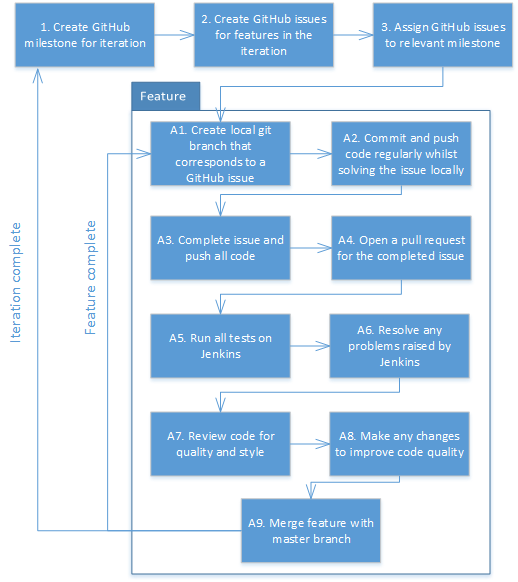
\includegraphics[scale=0.9]{Chapter2/git_workflow.png}
		\caption{The GitHub work flow diagram used for development. The outer processes (1-3) are performed for every iteration. The inner processes (A1-A9) are performed for every feature.}
		\label{fig:git_workflow}
	}
\end{figure}